\subsection{Problem 1}%
\label{sec:problem_1}
Solve the following system with the selected iterative solvers
\begin{equation*}
  \systeme{2u-v=0,-u+2v-w=0,-v+2w-z=0,-w+2z=5}
\end{equation*}
Estimate the computational costs and convergence rates.
Start the iterations from zero-value initial guess.
%%%%%%%%%%%%%%%%%%%%%%%%%%%%%%%%%%%%%%%%%%%%%%%%%%%%%%%%%%%%%%%%%%%%%%%%%%%%%%%
\subsubsection*{Mathematics}
%%%%%%%%%%%%%%%%%%%%%%%%%%%%%%%%%%%%%%%%%%%%%%%%%%%%%%%%%%%%%%%%%%%%%%%%%%%%%%%
The principle of the iterative linear solvers of the linear system of equations
expressed as $\matr{A}\matr{x}=\matr{b}$ is to start with some initial guess
$\matr{x}^{(0)}$ and approximate the solution with each iteration.

Stationary basic iterative methods, such as those presented in~\nameref{sec:algorithms},
perform a linear transformation $\matr{G}$ of the initial guess $\matr{x}^{(0)}$ at each
iteration:
\begin{equation*}
  \matr{x}^{(k+1)} = \matr{G}\matr{x}^{(k)} + \matr{c}
\end{equation*}

For any starting guess $\matr{x}^{(0)}$ the iterations are convergent to the real
solution $\matr{x}^{*}$ if and only if all of the eigenvalues of $\matr{G}$ are smaller
than $1$.

Assuming we know the exact solution $\matr{x}^*$, we may define the
\textit{solution error} $e$:
\begin{equation*}
  e^{(k)} = {\left\lVert\matr{x}^{*}-\matr{x}^{(k)}\right\rVert}_2
\end{equation*}
The method converges if the solution error converges to zero:
\begin{equation}
  \label{eqn:convergence_criterion}
  \lim_{k\to\infty}{e^{(k)}} = 0
  \quad \text{if} \quad
  \rho\left(\matr{G}^{(k)}\right) < 1
\end{equation}
where $\rho$ is the \textit{spectral radius}:
\begin{equation*}
  \rho(\matr{G}) = \max_i{\lvert\lambda_i\rvert} = \lVert\matr{\Lambda}\rVert_2
\end{equation*}

Following~\cite{Zdunek}, the value of the solution error at the $k$-th iteration may be
calculated via:
\begin{equation}
  \matr{e}^{(k)} = \matr{G}^k * \matr{e}^{(0)}
\end{equation}

\begin{itemize}
  \item Gauss-Seidel\\
    
    $ \matr{A} = \matr{S} - \matr{T} $
    where $ \matr{S} $ is the lower triangular part of $ \matr{A} $ including the diagonal, and $ \matr{T} $ is the strict upper triangular part of $ \matr{A} $.

    The iterative formula for the Gauss-Seidel method is
    $ \matr{Sx}_{k+1} = \matr{Tx}_k + \matr{b}, $
    which can be rewritten as
    $ \matr{x}_{k+1} = \matr{Gx}_k + \matr{c}, $
    where $ \matr{G} = \matr{S}^{-1}\matr{T} $ and $ \matr{c} = \matr{S}^{-1}\matr{b} $.

    The convergence of the Gauss-Seidel method is determined by the spectral radius of $ \matr{G} $, denoted by $ \rho(\matr{G}) $. The method converges if $ \rho(\matr{G}) < 1 $.

    To find $ \rho(\matr{G}) $, we first decompose $ \matr{A} $ into $ \matr{D} $, $ \matr{L} $, and $ \matr{U} $, where $ \matr{D} $ is the diagonal of $ \matr{A} $, $ \matr{L} $ is the strict lower triangular part of $ \matr{A} $, and $ \matr{U} $ is the strict upper triangular part of $ \matr{A} $. Then, we compute $ \matr{G} $ as follows:
    $ \matr{G} = (\matr{D} + \matr{L})^{-1}\matr{U}. $

    The spectral radius $ \rho(\matr{G}) $ is the maximum absolute value of the eigenvalues of $ \matr{G} $, given by
    $ \rho(\matr{G}) = \max_i |\lambda_i|, $
    where $ \lambda_i $ are the eigenvalues of $ \matr{G} $.

    Given a matrix $ \matr{A} $, the spectral radius $ \rho(\matr{G}) $ for the Gauss-Seidel method was calculated to be approximately 0.6, indicating that the iterations will converge.
      
  \item Successive Over-Relaxation \\

    SOR method is an improvement over the Gauss-Seidel method, it introduces a relaxation parameter $ \omega $ to accelerate convergence or correct overshooting of the function.
    For $\omega = 1$ method simplifies to Gauss-Seidel.

    The iteration scheme for the SOR method is given by:
    $$ \matr{x}_{k+1} = (1-\omega)\matr{x}_k + \omega \matr{D}^{-1}(\matr{b} - (\matr{L} + \matr{U})\matr{x}_k), $$
    where $ \matr{D} $ is the diagonal, $ \matr{L} $ is the strict lower triangular, and $ \matr{U} $ is the strict upper triangular part of the matrix $ \matr{A} $, and $ \omega $ is the relaxation factor such that $ 0 < \omega < 2 $.

    The matrix $ \matr{A} $ is split as $ \matr{A} = \matr{D} - \matr{L} - \matr{U} $, and the SOR iteration matrix $ \matr{G}$ is defined as:
    $$ \matr{G}  = (\matr{D} - \omega \matr{L})^{-1}[(1-\omega)\matr{D} + \omega \matr{U}]. $$

  \item Jacobi \\
  
    For the Jacobi method, the splitting of matrix $ \matr{A} $ is slightly different:
    $ \matr{A} = \matr{D} - \matr{R}, $
    where $ \matr{D} $ is the diagonal part of $ \matr{A} $, and $ \matr{R} $ is the remainder of $ \matr{A} $ (i.e., $ \matr{R} = \matr{L} + \matr{U} $).

    The iteration formula for the Jacobi method is:
    $ \matr{Dx}_{k+1} = \matr{Rx}_k + \matr{b}, $
    which can be rearranged to get the new estimate of $ \matr{x} $ at each iteration:
    $ \matr{x}_{k+1} = \matr{D}^{-1}(\matr{b} - \matr{Rx}_k). $

    In this case, the iteration matrix $ \matr{G} $ for the Jacobi method is defined as:
    $ \matr{G} = \matr{D}^{-1}\matr{R}. $

    The spectral radius of the iteration matrix, $ \rho(\matr{G}) = 0.8090$

  \item Landwebber \\
  
  The convergence of the Richardson's first-order method, depends on the appropriate choice of the relaxation parameter \( \alpha \). 
  For a given matrix $\matr{A}$, the iterations converge to the least-squares solution \( x = A^+b \) if \( \alpha \) is chosen within the range:
  \begin{equation*}
    0 < \alpha < 2|\lambda_{max}(\matr{A}^T\matr{A})| 
  \end{equation*}

  where  $\lambda_{max}(\matr{A}^T\matr{A})$ is the largest eigenvalue of $ \matr{A}^T\matr{A} $.

  Given the matrix $\matr{A}$ used in previous sections, we compute $\max{A}^T\matr{A}$ and then find its eigenvalues. 
  The maximum eigenvalue from this set determines the upper limit for the relaxation parameter. 
  
  The calculation is as follows:
  \begin{enumerate}
      \item Compute $ \matr{A}^T\max{A} $:
      \begin{equation*}
          A^TA = \matr{A}^\top \matr{A}
      \end{equation*}
      
      \item Find the eigenvalues of $\matr{A}^T\matr{A}$, denoted $\lambda_i$.
      
      \item Identify the maximum eigenvalue:
      \begin{equation*}
        \lambda_{max} = \max(\lambda_i)
      \end{equation*}
      
      \item Calculate the upper bound for \( \alpha \):
      \begin{equation*}
        \alpha < 2\lambda_{max}
      \end{equation*}
  \end{enumerate}

  Computed result using MATLAB gives us $\lambda_{max} \approx 13.0902$ giving us resulting convergence criterion range as:
  \begin{equation*}
    0 < \alpha < 0.1528
  \end{equation*}

  Choosing \( \alpha \) within this range ensures that the Landweber iterations will converge.

  \item Kaczmarz \\
  
    The convergence criterion for the Kaczmarz method is that the matrix $ \matr{A} $ must have no zero rows, 
    which ensures that each equation contributes to the determination of the solution. \\
    Additionally, for the method to converge, the following condition should be satisfied: 
    $ \matr{Ax} = \matr{b} $ must be consistent, meaning that at least one solution exists.
\end{itemize}
%%%%%%%%%%%%%%%%%%%%%%%%%%%%%%%%%%%%%%%%%%%%%%%%%%%%%%%%%%%%%%%%%%%%%%%%%%%%%%%
\subsubsection*{Solving}



%%%%%%%%%%%%%%%%%%%%%%%%%%%%%%%%%%%%%%%%%%%%%%%%%%%%%%%%%%%%%%%%%%%%%%%%%%%%%%%
\subsubsection*{Solution}
%%%%%%%%%%%%%%%%%%%%%%%%%%%%%%%%%%%%%%%%%%%%%%%%%%%%%%%%%%%%%%%%%%%%%%%%%%%%%%%
Since the considered system of linear equations is simple and consistent, we may use the
\MATLAB's backslash operator in the form of \lstinline[style=Matlab-editor]{A\b}, to
determine the exact solution:
\lstinputlisting[linerange={1-16},style=Matlab-editor]{problems/Problem_1.m}
\begin{equation*}
  \matr{A} = \begin{bmatrix}
    \phantom{-}2 & -1 & \phantom{-}0 & \phantom{-}0 \\
    -1 & \phantom{-}2 & -1 & \phantom{-}0 \\
    \phantom{-}0 & -1 & \phantom{-}2 & -1 \\
    \phantom{-}0 & \phantom{-}0 & -1 & \phantom{-}2
  \end{bmatrix}, \qquad
  \matr{b} = \begin{bmatrix}
    0 \\
    0 \\
    0 \\
    5
  \end{bmatrix}, \qquad
  \matr{x}^* = \begin{bmatrix}
    1 \\
    2 \\
    3 \\
    4
  \end{bmatrix}
\end{equation*}
Throughout solving this problem we attempt to use all the methods described in
the~\nameref{sec:algorithms}.
Before proceeding with approximating the solution, we want to check if the given method
converges.
To do so we verify~\autoref{eqn:convergence_criterion}:
\lstinputlisting[linerange={21-57},style=Matlab-editor]{problems/Problem_1.m}
Since all of our methods converge, we proceed with the approximation:
\lstinputlisting[linerange={59-69},style=Matlab-editor]{problems/Problem_1.m}
\begin{figure}[H]
  \centering
  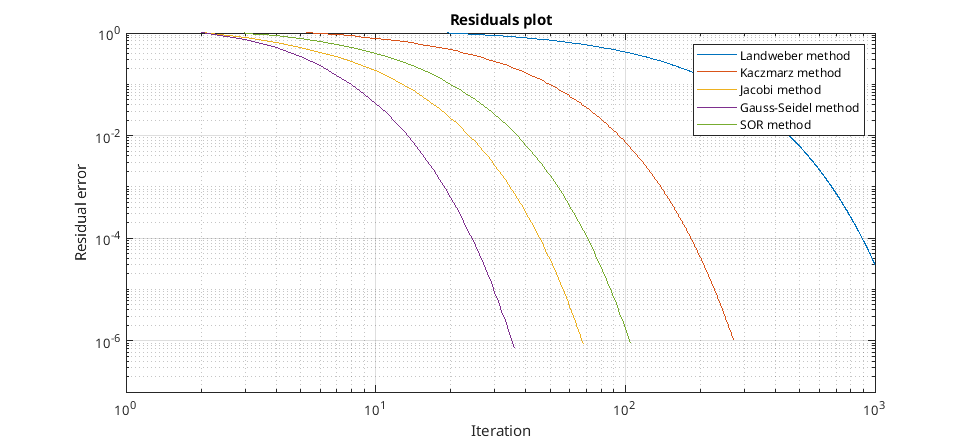
\includegraphics[width=1\textwidth]{images/Residuals_Problem1.png}
  \caption{Residuals of methods in problem 1}
\end{figure}